\documentclass[12pt]{article}

\title{Research proposal ELPP}
\author{Wessel Stoop, s0808709}

\usepackage{covington}
\usepackage{graphicx}
\usepackage{natbib}
\usepackage{float}

\renewcommand{\familydefault}{\sfdefault}

\let\stdsection\section
\renewcommand\section{\newpage\stdsection}

\begin{document}
\maketitle

\section{Introduction}
In a lot of cases, possibly even most cases, we do not say exactly what we want to convey. Sentence \ref{cold}, for example, can easily convey an order to close the window, and sentence \ref{hungry} could be a request for a sandwhich.

\begin{examples}
\item It's cold here. \label{cold}
\item Man, I'm hungry. \label{hungry}
\end{examples}

It is equally well possible, however, that sentence \ref{cold} is a request to leave, or that sentence \ref{hungry} is a suggestion to stop working and have a break. In pragmatic literature, where many similar examples can be found, these non-literal meanings are called the \emph{illocutionary force} \citep{a75}. \\\indent
But if we use indirect wordings like these all the time, how are we able to know what others mean? An answer many linguists (for example, \citet{c96,t08}) give to this question is the concept of \emph{common ground}. Common ground is the knowledge all conversation partners have, and know they all have. On the basis of this common ground, an addressee is able reconstruct the intention behind a particular utterance, and thus what the speaker really wanted to convey. This in turn allows the speaker to make his/her utterance shorter, or indirect (if one wants to be polite, for instance). Because of common ground, it is sometimes even possible to leave out language completely; a simple gesture is enough. This example, taken from \citet[pp. 3-5]{t08}, illustrates how powerful the common ground is:

\begin{quote}
Suppose that you and I are walking to the library, and out of the blue I point for you in the direction of some bicycles leaning against the library wall. [If] some days earlier you broke up with your boyfriend in a particularly nasty way, and we both know this mutually, and one the bicycles is his, which we also both know mutually, then [the pointing gesture might mean] "Your boyfriend's already at the library (so perhaps we should skip it)." On the other hand, if one of the bicycles is the one that we both know mutually was stolen from him recently, then the exact same pointing gesture will mean something completely different. [However, if] I am your friend from out of town and there is no way I could be familiar with your ex-boyfriend's bicycle, then you will not assume that I am indicating it for you. This is true even if, by some miracle, I do indeed know that this is his bicycle, but you do not know that I know this. In general, for smooth communication it is not enough that you and I each know separately and privately that this is his bicycle (and even that the other knows this); rather, this fact must be mutually known common ground between us. And in the case in which it is common ground between us that this is his bicycle, but not that the two of you have just broken up (even if we each know this privately), then you will probably think that I am indicating your boyfriend's bicycle as a way of encouraging our entrance into the library.
\end{quote}

According to Tomasello, if common grond is such an important part of language and communication in general, it must also be important to language acquisition. In fact, it might even be central to it: if, in the above example, the one who points at the bike would have uttered 'gavagai', the other person might be able to figure out that this could mean something like "let's not go in", solely on the basis of common ground.\\\indent
This does not necessarily mean infants and toddlers make complicated assumptions on the basis of shared experiences, as in the example above, however. Common ground can be as simple as both looking at the same thing, and both know that you are looking at this thing. This concept, common ground based on the immediate perceptual environment, is called \emph{joint attention}. So to translate the examples we started with into a language acquisition environment, a toddler hearing sentence \ref{hungry} might be able to figure out what 'hungry' means because he and his mother are both looking at a sandwhich. That is, joint attention can reduce referential uncertainty, and thus be a useful tool for language acquisition.\\\indent
Tomasello is not the first scholar to point out the importance of joint attention for language acquisition; the concept was first mentioned by \citet{b75}, and was investigated by various scholars afterwards. Much work related to the correlation between responsiveness to joint attention bids and language development has been done: there seems to be a positive correlation between joint attention abilities of 6-, 8-, 10-, 12-, and 18-month olds and later language abilities \citep{m00, c98} and infants who spent more time in joint attention activities with their mothers understood more language in the following months \citep{c98}. When approaching the matter from the opposite direction, it has been found that children with language development problems and autism often have joint attention impairments \citep{d02, m95, m86, od94, bc97}, and problems with joint attention can even be used as a predictor for autism \citep{m90}. Another popular topic is the difference between attention following and attention switching; it has been found that children who's mother had a tendency to follow the child's attention by talking about something the child was already looking at had a larger vocabulary than children who's mother tried to change the child's focus of attention \citep{c98,tt83}. \citet{ddc93} managed to replicate these findings in a controlled experiment: children who were taught the name of toys they were already looking at had a higher chance of remembering the name later than children who's attention was directed by the experimenter. \\\indent
An important focus in joint attention is the labeling of \emph{objects}: because joint attention reduces referential uncertainty, this is where its effects are expected to be the clearest. However, it is unclear whether findings concerning joint attention and objects can be generalized to language as a whole; the beginning of this introduction already indicated that language is much more complex than that, with its indirect utterances and assumptions one has to make about the intentions of the speaker. Do the advantages of joint attention for example carry over to learning verbs to refer to actions? \citet[pp. 312-313]{tk92} note: 

\begin{quote}
'The ostensive context may not work in this same way in the case of action words or verbs. First of all, we know very little about how children determine that an adult is using a word to refer to an action or process in an ostensive context [...]. Assuming that the child knows that an adult is referring to an action, the central joint attentional problem is that, unlike objects, actions are not permanent. Thus, in ostensive presentations of object labels the object remains in view throughout, so that the child may alternate attention between adult and object as needed. In ostensive presentations of verbs, on the other hand, the action is often transient — which means that the child gets only one brief chance to identify the intended action-referent and connect it to the new word, with no chance of attention alternation.'
\end{quote}

The study proposed here will investigate both the exact nature of joint attention, and whether any discovered effects also hold for actions. In section \ref{rq}, the research questions will be discussed in detail, and in section \ref{exp} it will be explained how this will be tested. In section \ref{expectations}, finally, the expected results will be discussed.

\section{Research questions} \label{rq}

The main research question for this research proposal is the following:

\begin{examples}
\item To what extent does \emph{joint attention} facilitate language learning?
\end{examples}

One can try to answer this question in many different ways, looking at it from many different angles. For this project, the question is split up into two subquestions. These questions will discussed in detail in the next two sections:

\subsection{What exactly is joint attention?}
Whereas some define joint attention as 'coordinating visual attention on external objects with an adult during social interaction', or something very similar (e.g. \citet{ddc93} and \citet{dd04}), others go further and define it as the 'immediate perceptual environment'-part of the common ground (e.g. \citet{c96} and \citet{t08}). The difference between these two definitions, although the writers may not have been fully aware of it, is that for the second defition conversation partners both have to know they are attending to the same thing, while this is not necessarily the case for the first one. From the addressee's perspective it would of course make sense to know what the speaker is attending to, because otherwise it might be hard to figure what his / her utterances relate to, but does this also hold for the speaker? Learning new words from eavesdropping on conversations does not seem that counter-intuitive, for example. And if it is indeed possible to learn new words from speaker that is not aware of what you are attending to, is this harder, and to what extent?\\\indent For clarity, joint attention in which all conversation participants are attending to the same thing AND know they are all attending to the same thing will be called \emph{strong joint attention}, whereas joint attention in which the speaker does not know where all addressees are attending to will be called \emph{weak joint attention}.

\subsection{Is joint attention also useful when learning action labels?}
As stated in the introduction, the literature on joint attention and language acquisition mostly focused on labeling objects. However, language entails much more than labeling objects, and it is questionable to what extant joint attention is also beneficial for other parts of language. In this research project, the focus will be one such other part: describing actions.

\section{The experiment} \label{exp}

This experiment tries to mimic the methodology of \citet{ddc93}, one of the few studies investigating joint attention experimentally, as closely as possible. This is true in particular for the procedure, the materials and the setting.

\subsection{Experimental design}

The experiment is set up in a way that it can provide evidence for both questions at the same time. This is possible, because both questions correspond to a factor in the design. \\\indent
For the first question (\emph{What exactly is joint attention?}), the factor \emph{type of joint attention} will be used. This factor consists of three groups: the \textbf{strong joint attention} group, which will be taught words while the speaker is attending to something together with the participant, the \textbf{weak joint attention} group, which will be listening to a conversation without taking part in it, and the \textbf{control} group, which will be learning words from a television screen showing pictures, without communication. The relevant characteristics of these groups can be summarized in table \ref{jagroups}.

\begin{table}[h] 
\begin{tabular}{|l||l|l|} 
\hline
&Strong joint attention&Weak joint attention\\
\hline
\hline
Strong joint attention group&+&+\\
\hline
Weak joint attention group&-&+\\
\hline
Control group&-&-\\
\hline
\end{tabular}
\caption{Characteristics of the three groups in the factor \emph{type of joint attention}.}
\label{jagroups}
\end{table}

The control group is necessary to be able to compare any discovered differences between the two types of joint attention to a non-joint attention situation. If a difference is found between the results of the two joint attention groups, the results of the control group indicate whether this is a large difference or not. If the results for the control group are much worse than both joint attention groups, one can conclude that both types of joint attention are beneficial, whereas one can conclude that only strong joint attention is beneficial if the results of the weak joint attention group pair with the results of the control group.\\\indent
For the second question, the factor \emph{type of concept} will be used. This factor consists of two groups: in one group, the participants will be taught words for objects, in the other group, the participants will be taught words for actions. \\\indent
This gives us six groups of participants, as is exemplified in table \ref{overview}.

\begin{table}[h] 
\begin{tabular}{|l||l|l|}
\hline
&Objects&Actions\\
\hline
\hline
Strong joint attention group&Group 1&Group 2\\
\hline
Weak joint attention group&Group 3&Group 4\\
\hline
Control group&Group 5&Group 6\\
\hline
\end{tabular}
\caption{Overview of the experimental design.}
\label{overview}
\end{table}

The participants will be randomly assigned to one of these groups. To investigate whether the differences between groups are significant, multifactorial ANOVA for independent measures can be used.

\subsection{Procedure}

The procedure will be dependent on the group the participant is in, and will therefore be described separately.\\\\\indent
\textbf{Group 1 and 2}
\begin{enumerate}
\item Participants play with their mother, to get used to the environment.
\item Participants play with the experimenter, to get used to the experimenter.
\item The experimenter introduces a new word to the participant.
\item A 3 minute break, in which the participant plays alone.
\item The participants are brought to the eye tracking device, and do the eye-tracking experiment.
\end{enumerate}

\textbf{Group 3 and 4}
\begin{enumerate}
\item Participants play with their mother, to get used to the environment.
\item Participants play with the experimenter, to get used to the experimenter.
\item Another experiment comes in, kneels so that the child can see him / her. The experimenter already present introduces a new word to the new experimenter. Both experimenters do not make contact with the participant during this stage.
\item A 3 minute break, in which the participant plays alone.
\item The participants are brought to the eye tracking device, and do the eye-tracking experiment.
\end{enumerate}

\textbf{Group 5 and 6}
\begin{enumerate}
\item The participant watches a television screen, on which an object or an action is shown. Together with the object or action, a pre-recorded sentence is played.
\item The participants are brought to the eye tracking device, and do the eye-tracking experiment.
\end{enumerate}

\subsection{Materials}
\paragraph{Word.} The actual word taught to the participants can be any pseudoword that is not too long or hard to pronounce; it is more important that the same word is used consistently for all groups. The word \emph{dodo}, as used by \citet{ddc93}, could be used, for instance.
\paragraph{Action.} For the action (group 2, 4 and 6), it is important that participant has not yet associated another label with it, making things like jumping or sliding inappropriate. A possible action could be waving the toy in circles. It is important that the action is repeated with multiple toys, so the child does not associate the actual object with the label. 
\paragraph{Toys.} For the toys, items will be used for which the children cannot have a label already. To achieve this, very basic toys (for instance, balls and dolls) will be avoided, just as toys which a particular brand name associated with them (for instance, \emph{Duplo} or \emph{Barbie}).
\paragraph{Video.} The video watched by group 5 and 6 contains either one animation-sentence pair (for group 5), or multiple ones (for group 6). The animations for group 6 are all different objects doing the same action (moving in circles). The pre-recorded sentence played while showing the animations should be something to keep the participants focussed; for example 'Look! It's a dodo!' or 'Look! He's dodoing!'.
\paragraph{Eye tracking experiment. } The eye tracking experiment consists of multiple 'scenes', each consisting of two animations, and one on the right. While these scenes are shown, a pre-recorded sentence is played. The eye tracking device registers at which of the animations the child looks. One of these scenes will contain the object / action for which the participant was taught a label. The other scenes are simple fillers, and can be anything that will keep the participant interested.

\subsection{Participants}
As participants, infants are needed who (1) are not too old, so they not know an other word for the toy or action already but also (2) are not too young, because they have to be sensitive to joint attention. The exact time at which this sensitivity develops is subject to debate (see \citet{dd04}), but there seems to be a consensus that joint attention is fully developed around the first year (regardless of when it started), as claimed by \citet{t92}, so for this research children from that age group will be chosen. \\\indent
Following \citet{ddc93}, each group will contain 15 participants. This means a total of 90 participants will be needed.

\subsection{Setting}
\begin{itemize}
\item For the joint attention task, the setting of the experiment will be a bright room with a carpet in the middle. On this carpet will be various toys, which can be used by the participant to play with, or by the experimenters to teach the participant a new word. The entire room will be video-taped.
\item For the television task of the control group, participants will be in a dark room with a television screen. Participants can sit on the lap of their mothers while watching the screen and listening to the sounds.
\item For the eye-tracking task, all participants will be brought to a dark room with an eye-tracking device. Participants can sit on the lap of their mothers while watching the screen and listening to the sounds.
\end{itemize}

\section{Expectations} \label{expectations}

The eye-tracking device registers which part of the screen the participant is paying attention to. When the pre-recorded sentence is played, and the child pays most attention to the part of the screen corresponding to the sentence, it will be assumed the child has learned the noun or the verb correctly.\\\indent
It is expected that in all groups participants will be able to associate the correct label with the object or the action, but that the amount of participants able to make the correct association varies. For example, it is expected that groups with weak joint attention will do less good, and that groups with no joint attention will perform even worse. Furtermore, it expected that all groups in which the participants were taught a label for an action will perform worse than their object counterparts. These results could be visualized as follows:

\begin{figure}[htb]
\centering
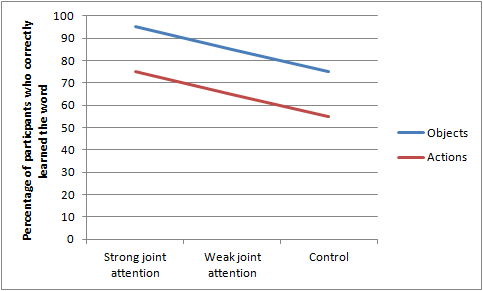
\includegraphics[width=0.8\textwidth]{graph_elpp.png}
\caption{The expected results}
\label{fig:results}
\end{figure}

If these results are found indeed, than we could conclude that joint attention has more advantages for learning nouns than for learning verbs, and that strong joint attention works best. Other likely results are that there is no difference between nouns and verbs, in which case the blue and red line in the graph will overlap, that there is no difference between weak and strong joint attention, in which case both lines will not go down from the first to the second point, or that there is difference between weak and no joint attention, in which case both lines will not go down from the second to the third point.

\section{Summary and conclusion} \label{sum}
In this research proposal, a study about joint attention was described. Joint attention will be investigated from two viewpoints. Firstly, participants will be divided into either a verb or a noun group, to investigate whether joint attention also facilitates learning words for actions. Secondly, participants will be divided into a strong joint attention group, a weak joint attention group and a control group. The strong joint attention group will be taught a word while the speaker and the participant are both attending to the same thing, the weak joint attention group will be overhearing a conversation by two experimenters, and the control group will be taught words by looking at a screen while listening to pre-recorded sentences. Expextations are that joint attention, in particular the strong form, will facilitate language learning, but that this will go best for nouns. This is expected because joint attention is so central for language learning and communication in general.

\begin{thebibliography}{99}
\bibitem[Austin(1975)]{a75}
Austin, J. L. (1975). \emph{How to do things with words.} Oxford: Oxford University Press. 
\bibitem[Baron-Cohen et al.(1997)]{bc97}
Baron-Cohen, S., D. A. Baldwin \& M. Crowson (1997). Do children with autism use the speaker’s direction of gaze strategy to crack the code of language? \emph{Child Development}, 68(1), 48 - 57.
\bibitem[Bruner(1975)]{b75} 
Bruner, J. (1975). The ontogenesis of speech acts. \emph{Journal of Child Language}, 2, 1 - 20.
\bibitem[Carpenter et al(1998)]{c98}
Carpenter, M., K. Nagell, \& M. Tomasello (1998). Social cognition, joint attention and communicative competence from 9 to 15 months of age. \emph{Monographs of the Society for Research in Child Development}, 63, 1 - 14.
\bibitem[Clark(1996)]{c96}
Clark, H. (1996). \emph{Uses of language.} Cambridge: Cambridge University Press.
\bibitem[Dawson et al.(2002)]{d02}
Dawson, G., J. Munson, A. Estes, J. Osterling, J. McPartland, K. Toth, L. Carver, \& R. Abbot, (2002). Neurocognitive function and joint attention ability in young children with autism spectrum disorder versus developmental delay. \emph{Child Development}, 73(2), 345 - 358.
\bibitem[Dominey \& Dodane (2004)]{dd04}
Dominey, P. F. \& C. Dodane (2004). \emph{Journal of Neurolinguistics}, 17, 121 - 145.
\bibitem[Dunham, Dunham \& Curwin(1993)]{ddc93}
Dunham, P. J., F. Dunham, \& A. Curwin (1993). Joint-attentional states and lexical acquisition at 18 months. \emph{Developmental Psychology}, 29(5), 827 - 831.
\bibitem[Morales et al.(2000)]{m00}
Morales, M., P. Mundy, C. E. F. Delgado, M. Yale, D. Messinger, R. Neal \& H. K. Schwartz (2000). Responding to joint attention across the 6- through 24-month age period and early language acquisition. \emph{Journal of Applied Developmental Psychology}, 21(3), 283 - 298.
\bibitem[Mundy(1995)]{m95}
Mundy, P. (1995). Joint attention and social-emotional approach behavior in children with autism. \emph{Development and Psychopathology}, 7, 63 - 82.
\bibitem[Mundy et al.(1990)]{m90}
Mundy, P., M. Sigman, \& C. Kasari (1990). A longitudinal study of joint attention and language development in autistic children. \emph{Journal of Autism and Developmental Disorders}, 20(1), 115 - 128.
\bibitem[Mundy et al.(1986)]{m86}
Mundy, P., M. Sigman, J. Ungerer, \& T. Sherman (1986). Defining the social deficits of autism: the contribution of nonverbal communication measures. \emph{Journal of Child Psychology and Psychiatry}, 27, 657 - 669.
\bibitem[Osterling \& Dawson(1994)]{od94}
Osterling, J., \& G. Dawson (1994). Early recognition of children with autism: a study of first birthday home video-tapes. \emph{Journal of Autism and Developmental Disorders}, 24, 247 - 257.
\bibitem[Tomasello(1992)]{t92}
Tomasello, M. (1992). The social bases of language acquisition. \emph{Social Development}, 1, 67 - 87.
\bibitem[Tomasello(2008)]{t08}
Tomasello, M. (2008). \emph{Origins of Human Communication.} Cambridge: MIT Press.
\bibitem[Tomasello \& Kruger(1992)]{tk92}
Tomasello, M. \& A. Kruger (1992). Joint attention on actions: acquiring verbs in ostensive and nonostensive contexts. \emph{Journal of Child Language} 19, 311 - 333.
\bibitem[Tomasello \& Todd(1983)]{tt83}
Tomasello, M., \& J. Todd (1983). Joint attention and lexical acquisition style. \emph{First Language}, 4, 197 - 212.
\end{thebibliography}

\end{document}